% Our architecture in the visual language of the SAM2 paper figure (plots/nfo/model_diagram.png):
% green = image encoder, orange = mask decoder, lavender = prompt encoder, pink = memory (not used).
% Blue outline = trained by us. Natural width ≈ 20 cm; the poster scales it to the column width.
\providecommand{\ArchSub}{\fontsize{14}{16}\selectfont}
% trained (flame) / frozen (snowflake) markers, drawn so they work with pdfLaTeX and XeTeX alike
\newsavebox{\FireBox}\newsavebox{\IceBox}
\sbox{\FireBox}{\tikz[baseline=-0.1em, x=0.9em, y=0.9em]{%
  \fill[orange!90!red] (0,-0.5) .. controls (-0.55,-0.25) and (-0.35,0.25) .. (0,0.75)
                       .. controls (0.35,0.25) and (0.55,-0.25) .. (0,-0.5);
  \fill[yellow!85!orange] (0,-0.45) .. controls (-0.25,-0.25) and (-0.15,0.05) .. (0,0.25)
                          .. controls (0.15,0.05) and (0.25,-0.25) .. (0,-0.45);}}
\sbox{\IceBox}{\tikz[baseline=-0.1em, x=0.9em, y=0.9em, line width=0.12em, cyan!60!blue, line cap=round]{%
  \foreach \a in {0,60,120} {\draw (\a:-0.55) -- (\a:0.55);
    \draw (\a:0.32) -- ++(\a+35:0.18); \draw (\a:0.32) -- ++(\a-35:0.18);
    \draw (\a:-0.32) -- ++(\a+215:0.18); \draw (\a:-0.32) -- ++(\a+145:0.18);}}}
\providecommand{\Fire}{\usebox{\FireBox}}\providecommand{\Ice}{\usebox{\IceBox}}
\definecolor{SamEnc}{HTML}{D4F5C4}\definecolor{SamEncD}{HTML}{8FCF79}
\definecolor{SamDec}{HTML}{FDE6C8}\definecolor{SamDecD}{HTML}{E9B676}
\definecolor{SamPrm}{HTML}{DEDDFB}\definecolor{SamPrmD}{HTML}{9E9BE6}
\definecolor{SamMem}{HTML}{F9DDF0}\definecolor{SamMemD}{HTML}{E7A9D3}
\begin{tikzpicture}[x=1cm, y=1cm, font=\fontsize{19}{22}\selectfont,
    lab/.style={align=center, font=\fontsize{17}{20}\selectfont},
    small/.style={align=center, font=\fontsize{14}{16}\selectfont, text=black!70},
    blk/.style={rounded corners=7pt, line width=1.4pt, align=center, minimum height=1.9cm},
    ours/.style={blk, draw=ColOurs, fill=ColOurs!14, line width=2.6pt},
    stride/.style={draw=ColOurs, fill=white, rounded corners=4pt, line width=1.2pt, minimum width=2.3cm,
                   minimum height=1.1cm, font=\fontsize{15}{17}\selectfont},
    arr/.style={-{Latex[length=4mm, width=3mm]}, line width=1.8pt, draw=black!80},
    thin/.style={-{Latex[length=3mm, width=2.4mm]}, line width=1.2pt, draw=ColOurs},
    feat/.style={draw=SamEncD, fill=SamEnc!70, line width=1.1pt, minimum width=1.3cm, minimum height=1.3cm}]

  % inputs
  \node[inner sep=0pt] (X) at (-6, 0) {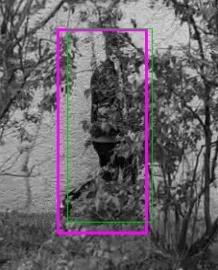
\includegraphics[height=4.2cm]{plots/nfo/inputs_0.jpg}};
  \node[inner sep=0pt] (C) at ( 0, 0) {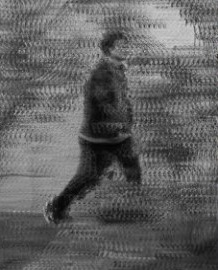
\includegraphics[height=4.2cm]{plots/nfo/inputs_2.jpg}};
  \node[inner sep=0pt] (B) at ( 6, 0) {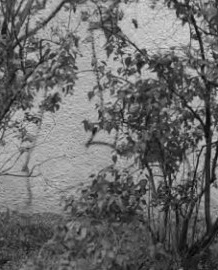
\includegraphics[height=4.2cm]{plots/nfo/inputs_1.jpg}};
  \node[lab, above=1mm of X] {\textbf{frame} $t$\\[-1mm]{\ArchSub with tracker box}};
  \node[lab, above=1mm of C] {\textbf{integral image}\\[-1mm]{\ArchSub 6 past frames, aligned}};
  \node[lab, above=1mm of B] {\textbf{empty scene}\\[-1mm]{\ArchSub encoded once per scene}};

  % shared image encoder (trapezoid, as in SAM2)
  \node[trapezium, trapezium angle=78, shape border rotate=180, draw=SamEncD, fill=SamEnc, line width=1.4pt,
        minimum width=18.5cm, minimum height=2cm, align=center] (enc) at (0, -3.9)
        {\Ice\ \textbf{image encoder}\\[-1mm]{\ArchSub same weights for all three}};
  \foreach \n/\x in {X/-6, C/0, B/6} \draw[arr] (\n.south) -- (\x, -2.9);

  % feature maps (strides 16 / 8 / 4)
  \foreach \n/\x/\t in {fx/-6/t, fc/0/I, fb/6/E} {
    \node[feat] at (\x+0.25, -6.5+0.25) {};
    \node[feat] (\n) at (\x, -6.5) {$F_{\t}$};
    \draw[arr] (\x, -4.9) -- (\n.north);
  }
  \node[small, anchor=west] at (7.0, -7.45) {strides\\16, 8, 4};

  % adapter: takes only the three feature maps; per stride, coarse to fine
  \node[ours, minimum width=15cm, minimum height=3.6cm] (ad) at (1, -9.9) {};
  \node[anchor=north west, align=left] at ([xshift=3mm, yshift=-2mm]ad.north west)
        {\Fire\ \textbf{adapter}\ \ {\ArchSub 0.7\,M parameters}};
  \node[stride] (s16) at (-3.2, -10.6) {stride 16};
  \node[stride] (s8)  at ( 0.9, -10.6) {stride 8};
  \node[stride] (s4)  at ( 5.0, -10.6) {stride 4};
  \draw[thin] (s16) -- (s8); \draw[thin] (s8) -- (s4);
  \foreach \n in {fx, fc, fb} \draw[arr] (\n.south) -- (\n.south |- ad.north);

  % corrections added to the frame features at each stride
  \node[circle, draw=black!80, line width=1.8pt, minimum size=1cm, inner sep=0pt,
        font=\fontsize{28}{28}\selectfont\bfseries] (plus) at (-9.6, -9.9) {$+$};
  \draw[arr] (fx.west) -| (plus.north);
  \draw[arr] (ad.west) -- node[above, small] {corrections} (plus.east);

  % decoder + prompt encoder
  \node[blk, draw=SamDecD, fill=SamDec, minimum width=7.2cm] (dec) at (-4.6, -13.6)
        {\Ice\ \textbf{mask decoder}};
  \node[blk, draw=SamPrmD, fill=SamPrm, minimum width=6.4cm] (pe) at (5, -13.6)
        {\Ice\ \textbf{prompt encoder}};
  \draw[arr] (plus.south) |- (dec.west);
  \draw[arr] (pe.west) -- (dec.east);
  \draw[arr, dashed] (pe.north |- ad.south) -- node[right, small] {point\\[-1mm]correction} (pe.north);

  % tracker: where to look
  \node[blk, draw=ColOurs, fill=white, line width=1.4pt, minimum width=6.4cm] (trk) at (5, -16.5)
        {\textbf{tracker}\\[-1mm]{\ArchSub motion + box: where to look}};
  \draw[arr] (trk.north) -- (pe.south);
  % tracker input: change of the frame features against the empty scene
  \draw[-{Latex[length=3mm, width=2.4mm]}, line width=1.2pt, draw=black!60] (fb.east) -- (9.2, -6.5) -- (9.2, -15.9)
        node[pos=0.5, rotate=-90, anchor=south, inner sep=1.5pt, small] {change of $F_t$ vs $F_E$} -- ([yshift=6mm]trk.east);
  % the tracker's motion builds the integral image
  \draw[arr, draw=ColOurs, dashed] (trk.east) -- ++(1.6, 0) |- ([yshift=3.4cm]C.north) node[pos=0.75, above, small, text=ColOurs]
        {motion: aligns the past frames} -- ([yshift=1.75cm]C.north);
  % legend
  \node[anchor=south west, align=left, font=\fontsize{16}{19}\selectfont] at (-11.6, -21.4)
        {\Fire\ trained (ours)\\ \Ice\ frozen SAM2.1};

  % output
  \node[inner sep=0pt] (M) at (-4.6, -18.1) {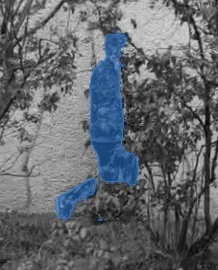
\includegraphics[height=4.2cm]{plots/nfo/inputs_6.jpg}};
  \draw[arr] (dec.south) -- (M.north);
  \node[lab, left=2mm of M] {\textbf{mask}};

  % memory path of SAM2: not used
  \node[blk, draw=SamMemD, fill=SamMem!50, dashed, minimum width=6.4cm, text=black!55] (mem) at (5, -19.4)
        {memory of past masks\\[-1mm]{\ArchSub not used}};
  \draw[arr, draw=black!35, dashed] (M.east |- mem.west) -- node[text=ColSamurai, font=\fontsize{30}{30}\selectfont\bfseries]
        {$\times$} (mem.west);
\end{tikzpicture}
